\begin{figure}[htbp]
\centering
\begin{tikzpicture}[x=1cm,y=1cm]
\node[anchor=south west,inner sep=0] at (0,0) {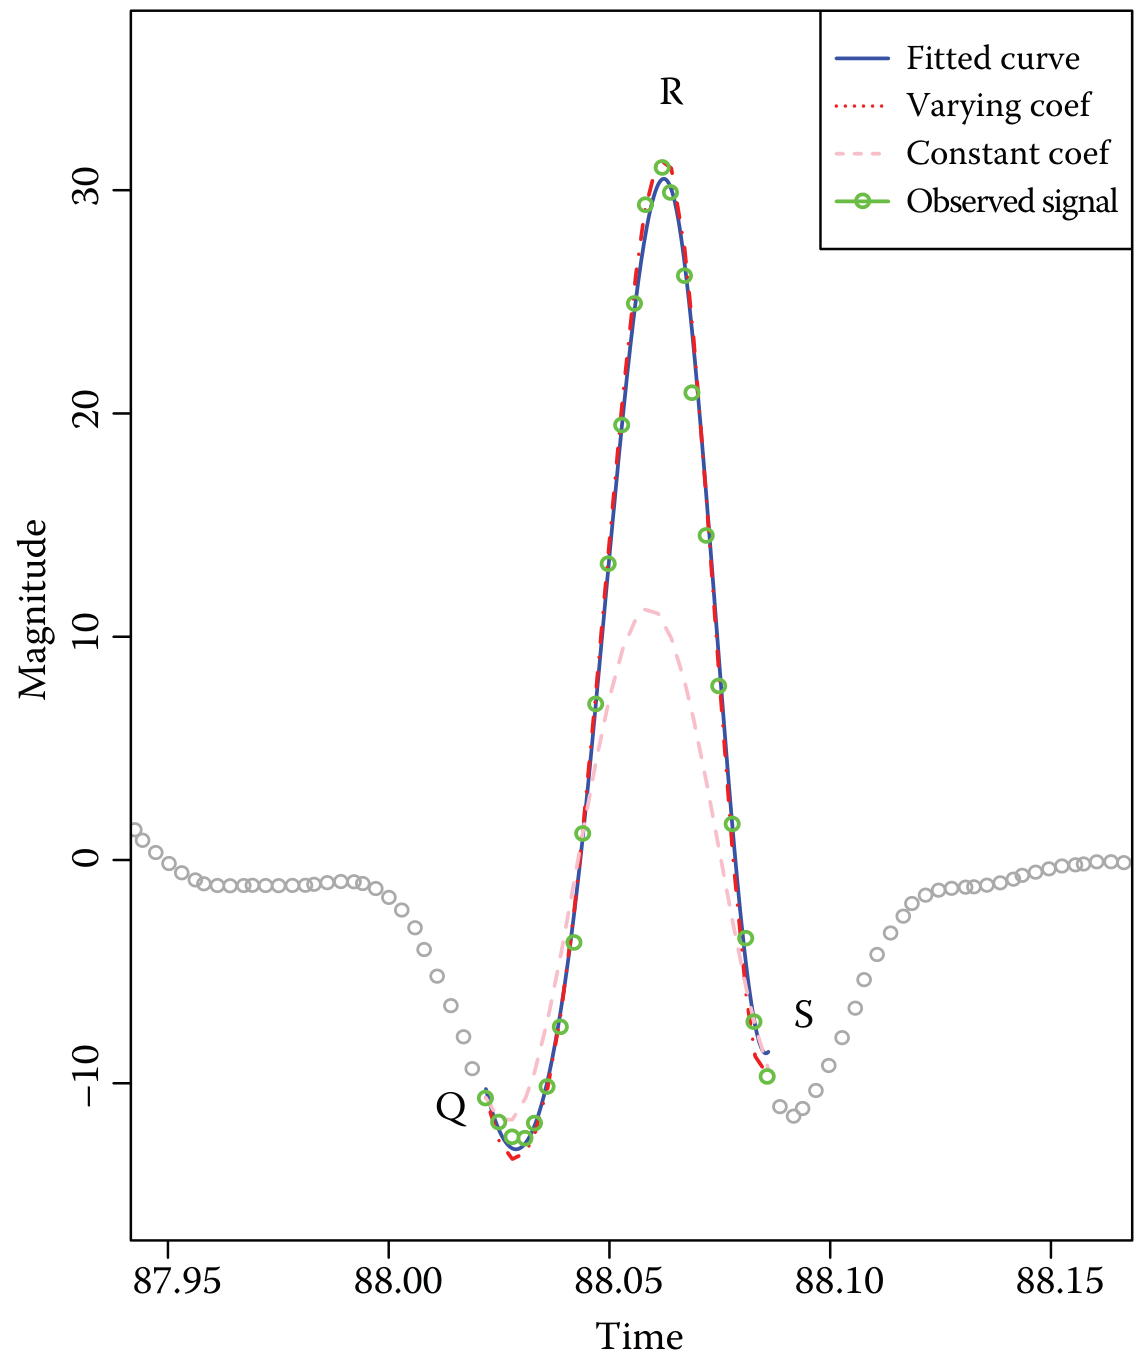
\includegraphics[width=10.5cm]{figures/ch03_fig03_data.png}};
\fill[white] (8.2895,10.3480) rectangle (10.3987,12.4941);
\fill[white] (5.4482,0.0817) rectangle (6.3258,0.4962);
\node[font=\scriptsize,rotate=0,inner sep=0] at (5.8870,0.2889) {时间};
\fill[white] (0.1063,6.1370) rectangle (0.5300,7.8634);
\node[font=\scriptsize,rotate=90,inner sep=0] at (0.3182,7.0002) {幅值};
\node[font=\scriptsize,rotate=0,inner sep=0] at (9.1469,12.0658) {拟合曲线};
\node[font=\scriptsize,rotate=0,inner sep=0] at (9.1909,11.6268) {时变系数};
\node[font=\scriptsize,rotate=0,inner sep=0] at (9.2775,11.1879) {常系数};
\node[font=\scriptsize,rotate=0,inner sep=0] at (9.3236,10.7489) {观测信号};
\end{tikzpicture}
\origfig{3}{二阶常微分方程拟合得到的曲线。}
\label{fig:ch03-03}
\end{figure}
